\appendix
\chapter{Curve di discriminazione}                          %imposta le appendici
Vengono di seguito riportate le curve di discriminazione dei vari fotomoltiplicatori dei piani di rivelazione 0 e 1.

\begin{figure}[H]
	\centering
		\begin{minipage}{.5\textwidth}
			\centering
			\subfloat[][]{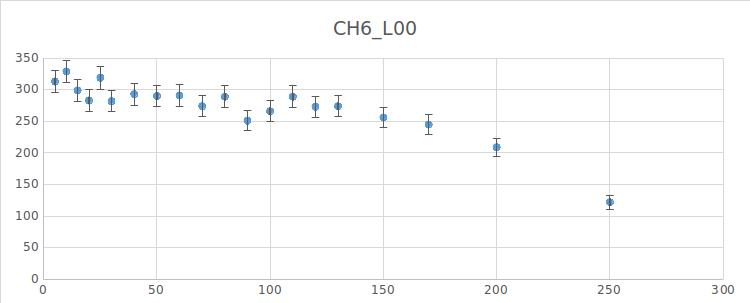
\includegraphics[width=1\textwidth]{excel-plots/disc-L00.jpg}\label{fig:disc-L00}}\quad
		\end{minipage}%
		\begin{minipage}{.5\textwidth}
			\centering
			\subfloat[][]{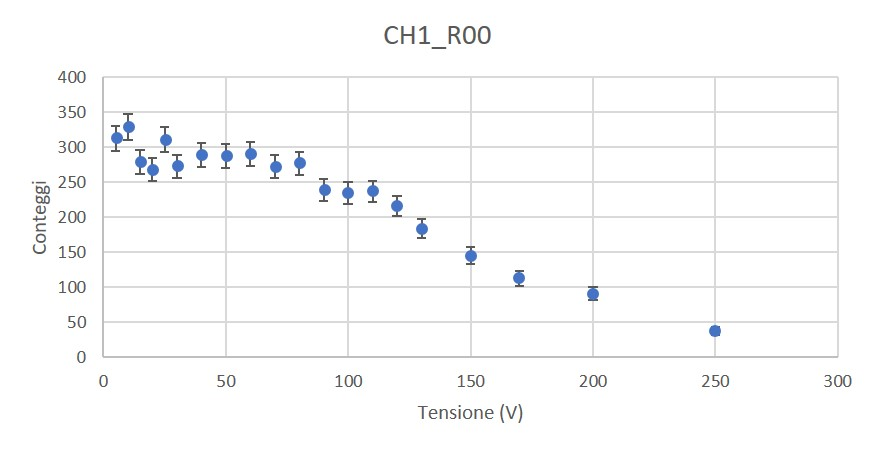
\includegraphics[width=1\textwidth]{excel-plots/disc-R00.jpg}\label{fig:disc-R00}}\quad
		\end{minipage}
	\begin{minipage}{.5\textwidth}
		\centering
		\subfloat[][]{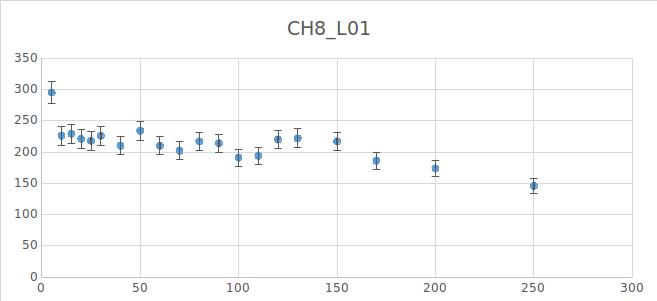
\includegraphics[width=1\textwidth]{excel-plots/disc-L01.jpg}\label{fig:disc-L01}}\quad
	\end{minipage}%
	\begin{minipage}{.5\textwidth}
		\centering
		\subfloat[][]{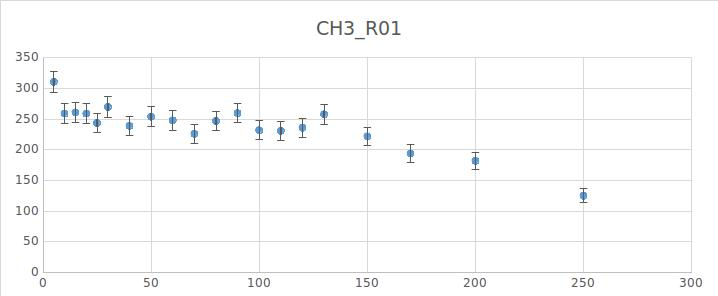
\includegraphics[width=1\textwidth]{excel-plots/disc-R01.jpg}\label{fig:disc-R01}}\quad
	\end{minipage}
  \caption{Curva di discriminazione dei PMT del piano 0, in particolare del PMT L00(a), R00(b), L10(c) e R10(d).}
\end{figure}

\begin{figure}[H]
	\centering
		\begin{minipage}{.5\textwidth}
			\centering
			\subfloat[][]{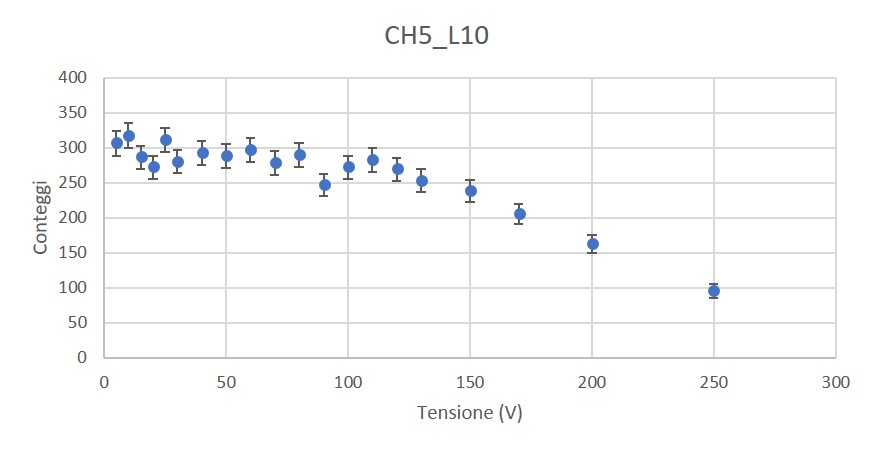
\includegraphics[width=1\textwidth]{excel-plots/disc-L10.jpg}\label{fig:disc-L10}}\quad
		\end{minipage}%
		\begin{minipage}{.5\textwidth}
			\centering
			\subfloat[][]{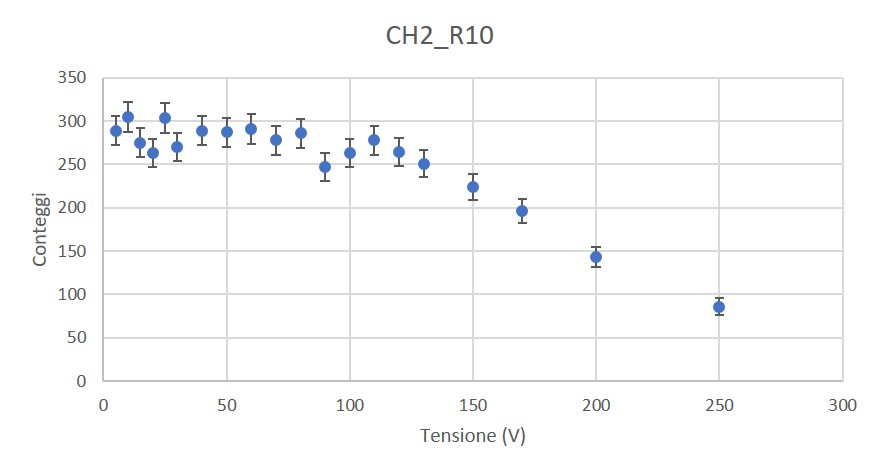
\includegraphics[width=1\textwidth]{excel-plots/disc-R10.jpg}\label{fig:disc-R10}}\quad
		\end{minipage}
		\begin{minipage}{.5\textwidth}
			\centering
			\subfloat[][]{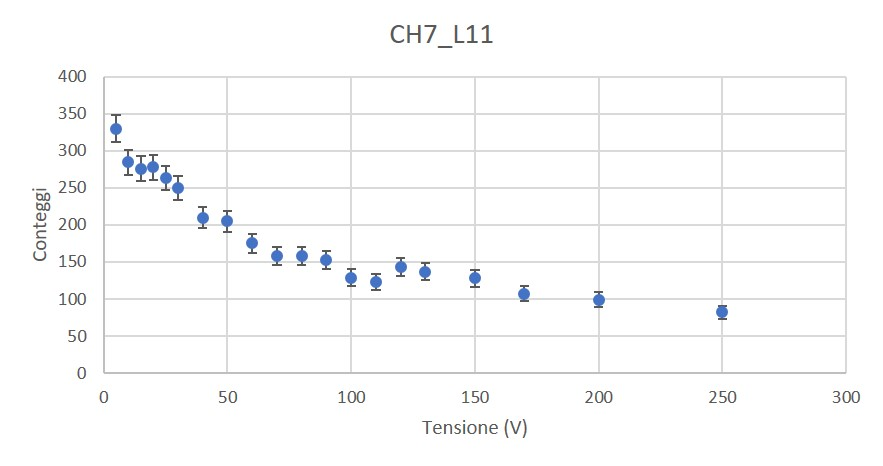
\includegraphics[width=1\textwidth]{excel-plots/disc-L11.jpg}\label{fig:disc-L11}}\quad
		\end{minipage}%
		\begin{minipage}{.5\textwidth}
			\centering
			\subfloat[][]{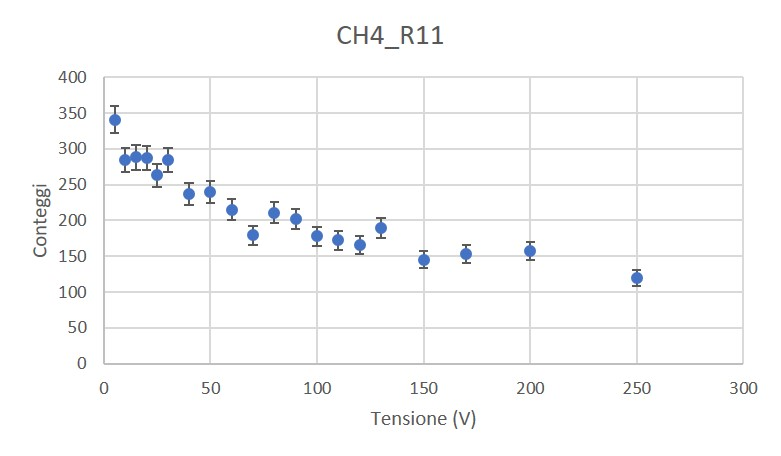
\includegraphics[width=1\textwidth]{excel-plots/disc-R11.jpg}\label{fig:disc-R11}}\quad
		\end{minipage}
    \caption{Curva di discriminazione dei PMT del piano 1, in particolare del PMT L01(e), R01(f), L11(g) e R11(h).}
\end{figure}


\chapter{Rette di calibrazione dei TDC}               %crea l'appendice
Vengono di seguito riportate le rette di calibrazione del Time to Digital Converter.

\begin{figure}[H]
  \centering
  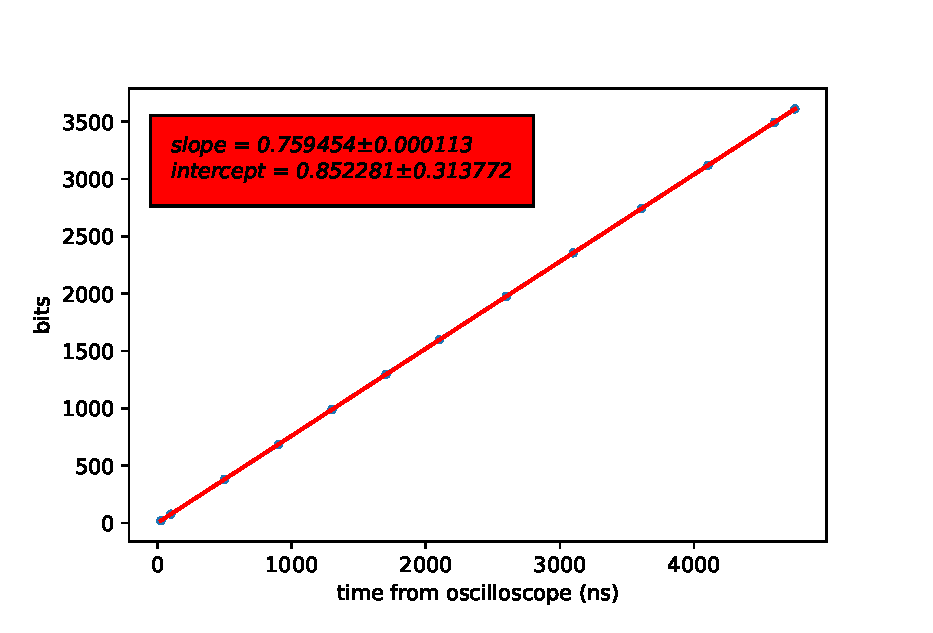
\includegraphics[width=.8\textwidth]{plots/tdc11.eps}
  \caption{Retta di calibrazione del canale 1 del TDC 1.}
  \label{fig:tdc11}
\end{figure}

\begin{figure}[H]
  \centering
  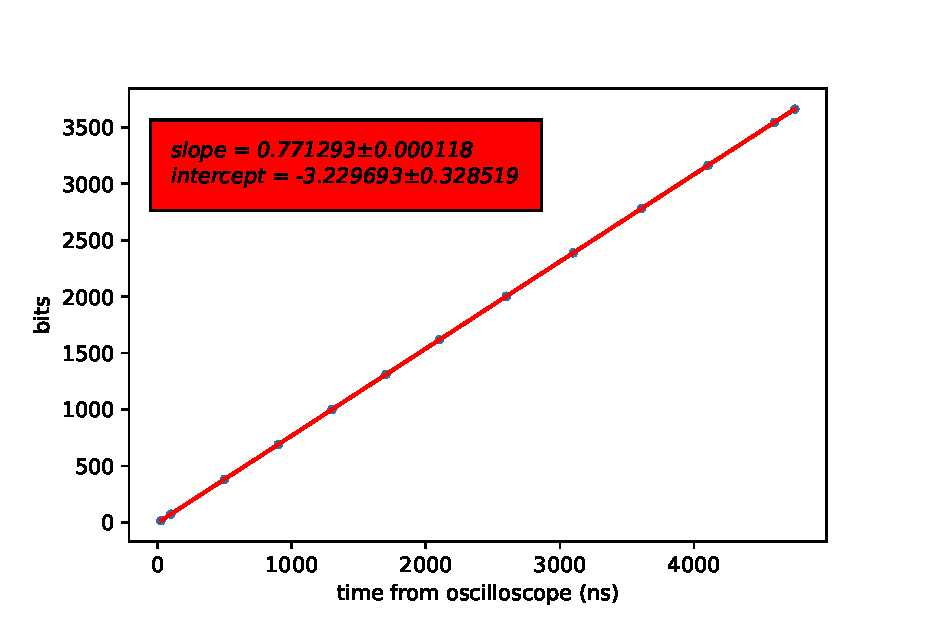
\includegraphics[width=.8\textwidth]{plots/tdc12.eps}
  \caption{Retta di calibrazione del canale 2 del TDC 1.}
  \label{fig:tdc12}
\end{figure}

\begin{figure}[H]
  \centering
  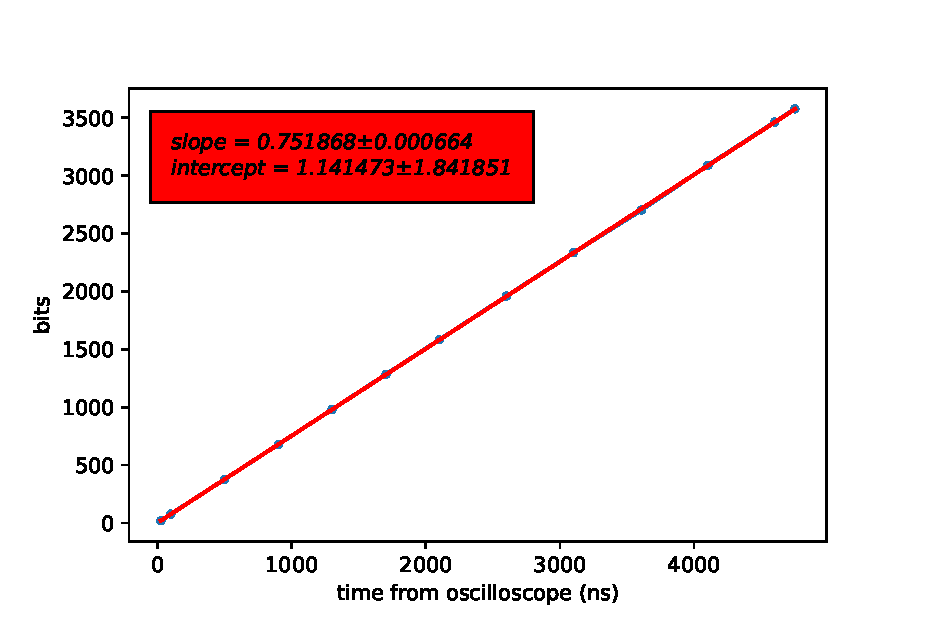
\includegraphics[width=.8\textwidth]{plots/tdc13.eps}
  \caption{Retta di calibrazione del canale 3 del TDC 1.}
  \label{fig:tdc13}
\end{figure}

\begin{figure}[H]
  \centering
  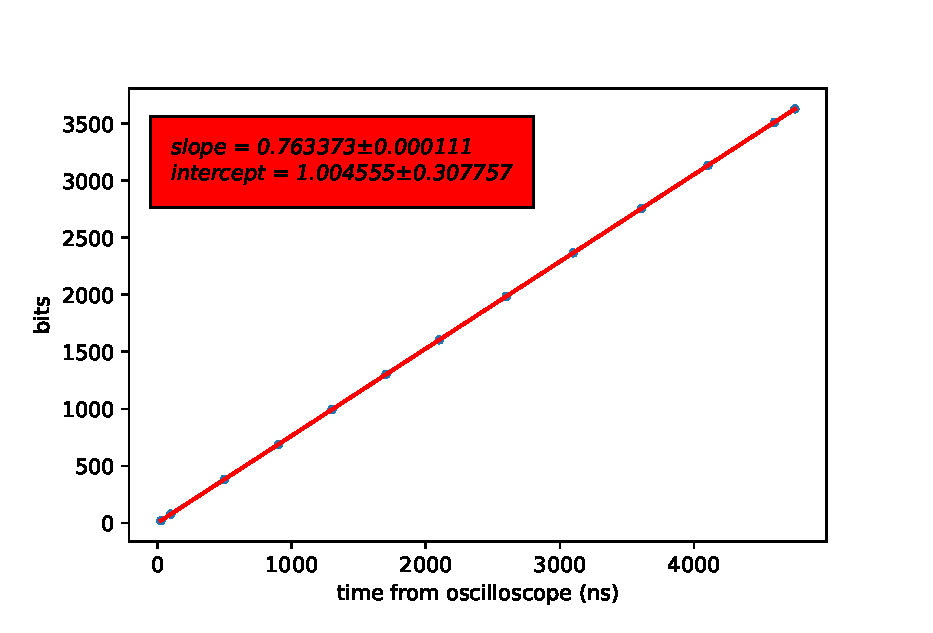
\includegraphics[width=.8\textwidth]{plots/tdc14.eps}
  \caption{Retta di calibrazione del canale 4 del TDC 1.}
  \label{fig:tdc14}
\end{figure}

\begin{figure}[H]
  \centering
  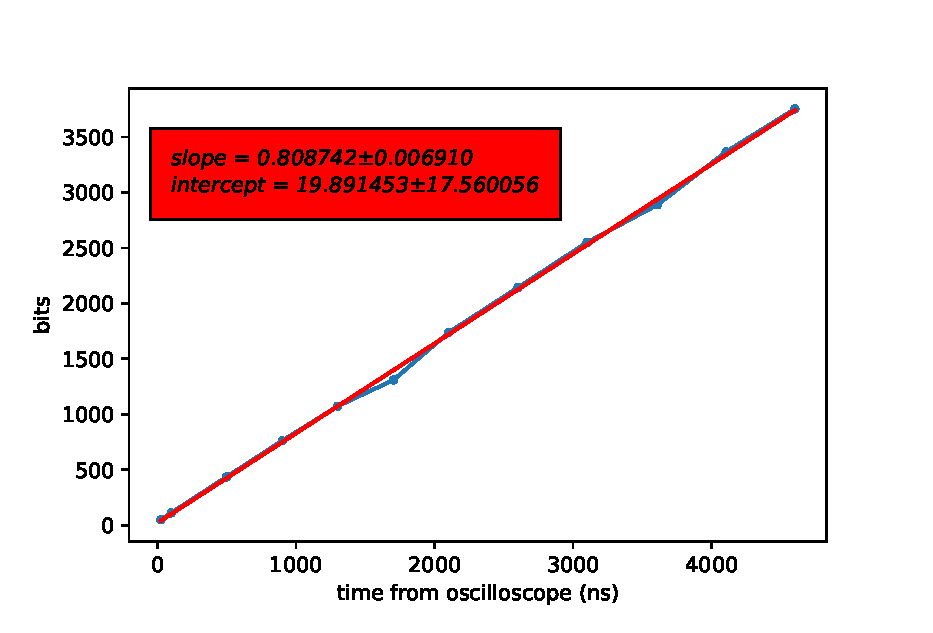
\includegraphics[width=.8\textwidth]{plots/tdc23.eps}
  \caption{Retta di calibrazione del canale 3 del TDC 2.}
  \label{fig:tdc23}
\end{figure}

\begin{figure}[H]
  \centering
  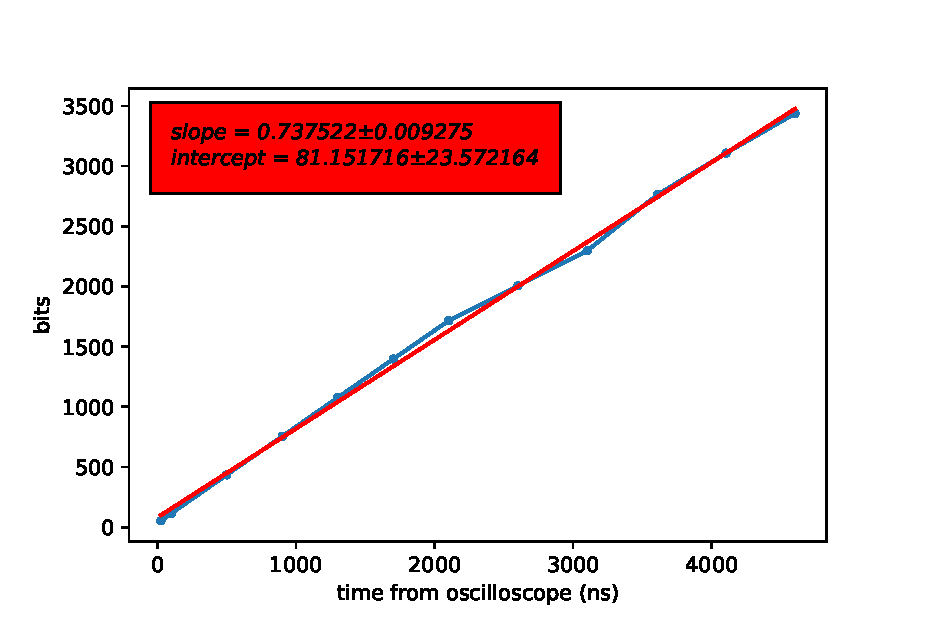
\includegraphics[width=.8\textwidth]{plots/tdc24.eps}
  \caption{Retta di calibrazione del canale 4 del TDC 2.}
  \label{fig:tdc24}
\end{figure}

\begin{figure}[H]
  \centering
  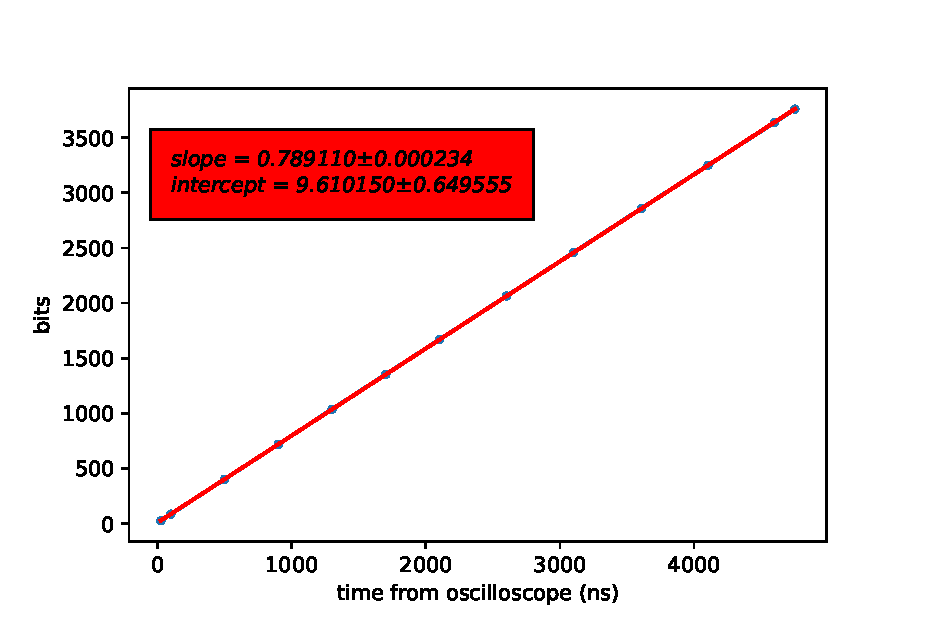
\includegraphics[width=.8\textwidth]{plots/tdc25.eps}
  \caption{Retta di calibrazione del canale 2 del TDC 5.}
  \label{fig:tdc25}
\end{figure}

\begin{figure}[H]
  \centering
  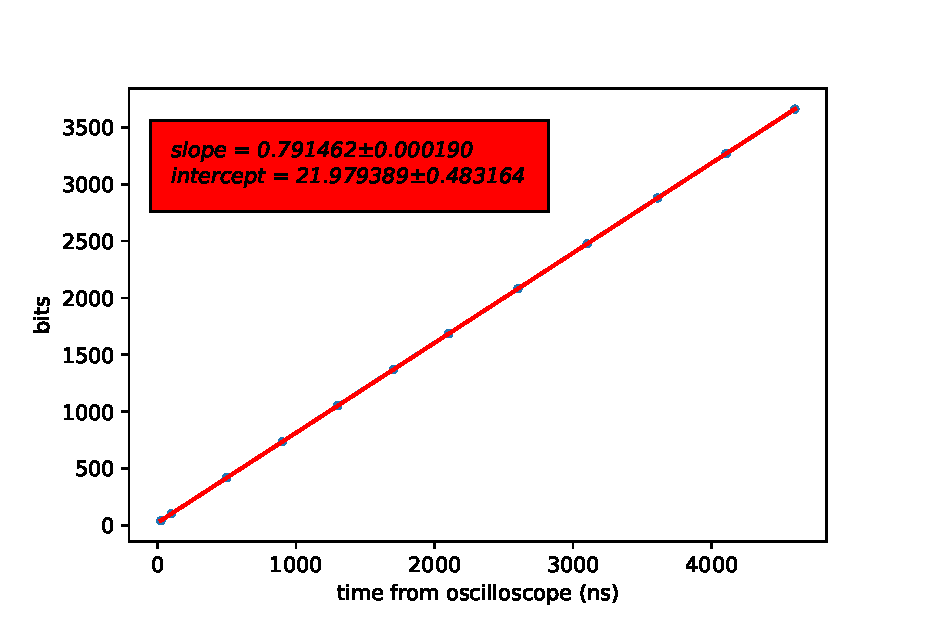
\includegraphics[width=.8\textwidth]{plots/tdc26.eps}
  \caption{Retta di calibrazione del canale 6 del TDC 2.}
  \label{fig:tdc26}
\end{figure}



%\rhead[\fancyplain{}{\bfseries \thechapter \:Prima Appendice}]
%{\fancyplain{}{\bfseries\thepage}}

\chapter{Energia depositata negli scintillatori}             %crea l'appendice

L'apparato di rivelazione utilizzato consiste di scintillatori plastici sottili. L'attesa \`e che l'energia persa dalle particelle che attraversano tale apparato segua una distribuzione di Landau.\\
Mentre per assorbitori relativamente spessi \`e comune osservare una distribuzione dell'energia trasferita essenzialmente gaussiana, nel caso di assorbitori sottili il valor medio della distribuzione \`e pi\`u grande del valore pi\`u probabile. Qualitativamente possiamo spiegare questo
scostamento osservando che al diminuire dello spessore di materiale bersaglio, calando il numero medio di urti, cresce la frequenza di eventi con grande trasferimento di energia della particella in una singola collisione. Tali eventi (knock on collisions) sono rari ma sufficienti ad
originare la coda asimmetrica tipica della distribuzione di Landau.
Per grandi spessori, viceversa, l'alto numero medio di urti permette di introdurre l'approssimazione dovuta al Teorema del Limite Centrale. In altri termini, eventi a grande trasferimento di energia sono sempre presenti ma statisticamente sommersi dagli altri.\\
Per verificare il corretto funzionamento dei rivelatori si \`e quindi deciso di misurare la quantit\`a di carica prodotta nei fotomoltiplicatori che \`e proporzionale all'energia depositata ed \`e data da:
\begin{equation}
Q=N_{\gamma}\times CE \times QE \times G
\end{equation}
dove:
\begin{itemize}
	\item $N_{\gamma}$ = numero di fotoni prodotti dalla particella nello scintillatore;
	\item CE = collection efficiency = percentuale di fotoni raccolti nello scintillatore che arrivano al fotocatodo ($\sim 80-90 \%$);
	\item QE = quantum efficiency = percentuale di fotoni che producono un foto-elettrone sul fotocatodo;
  \item G = gain = numero di elettroni prodotti alla fine della catena di moltiplicazione dei dinodi del PM per singolo fotoelettrone.
\end{itemize}
Il circuito utilizzato per effettuare questa misura \`e schematizzato in Figura \ref{fig:circ-energy}. Il trigger per la presa dati \`e costituito da un $\mu_{passante}$, ovvero un muone che non viene catturato dalla lastra di ferro per poi decadere, ma vi passa attraverso. Ci\`o si traduce in un segnale in coincidenza temporale sui tre scintillatori dei semi-piani anteriori:
\begin{equation}
  T (\mu_{passante})=(L00 \lor R00) \land (L10 \lor R10) \land (L20 \lor R20)
\end{equation}
La carica depositata sui tre scintillatori \`e misurata tramite un modulo CaMAC CIA (Charge Integrating ADC) il quale integra il segnale analogico in ingresso per un certo intervallo di tempo definito dalla lunghezza del segnale digitale sul GATE. Il segnale del Trigger viene dato in entrata a tre dual-timer:
\begin{enumerate}
	\item il primo viene allargato fino a 400ns e usato come GATE di presa di segnale del modulo CIA (ovvero viene messo in coincidenza con gli altri segnali in entrati in modo che i dati vengano presi solo mentre l'onda quadra \`e in un 1 logico, ovvero per un tempo che corrisponde alla sua larghezza);
	\item il secondo viene allargato fino a 1s e usato come veto dell'AND logico del trigger per dare il tempo al CIA di processare correttamente i segnali;
	\item dal terzo si prende l'end-marker allargato tramite un LED e ritardato di 1000 ns in modo che si collochi necessariamente dopo tutti i segnali e dopo il gate, ma comunque all'interno del tempo morto del veto. Questo segnale viene dato in input a uno dei canali del CIA (channel 7) in modo da risultare attivo, ma senza misurare nulla: ci\`o permette di fare una stima del rumore elettronico introdotto nel circuito.
\end{enumerate}

Gli altri canali del CIA sono riempiti dai segnali provenienti dai PM Left e Right degli scintillatori (channels 1-6), che vengono leggermente ritardati tramite un delay per compensare i ritardi introdotti nell'elettronica, o sono lasciati vuoti in modo da poter fare una stima del rumore termico presente nel circuito (channels 8-16).\\
Essendo il CIA un modulo CAMAC i dati sono stati acquisiti tramite un semplice programma in LabView. I risultati dell'analisi dei dati cos\`i raccolti forniscono, come ci si poteva aspettare, delle distribuzioni di Landau (vedi Figura \ref{fig:L00_energy} a titolo di esempio). Il Goodness of Fit test fornisce un risultato di $\chi^{2}/\text{DoF}=1.27$, a testimonianza della bont\`a del fit eseguito.

\begin{figure}[H]
 	\begin{center}
 		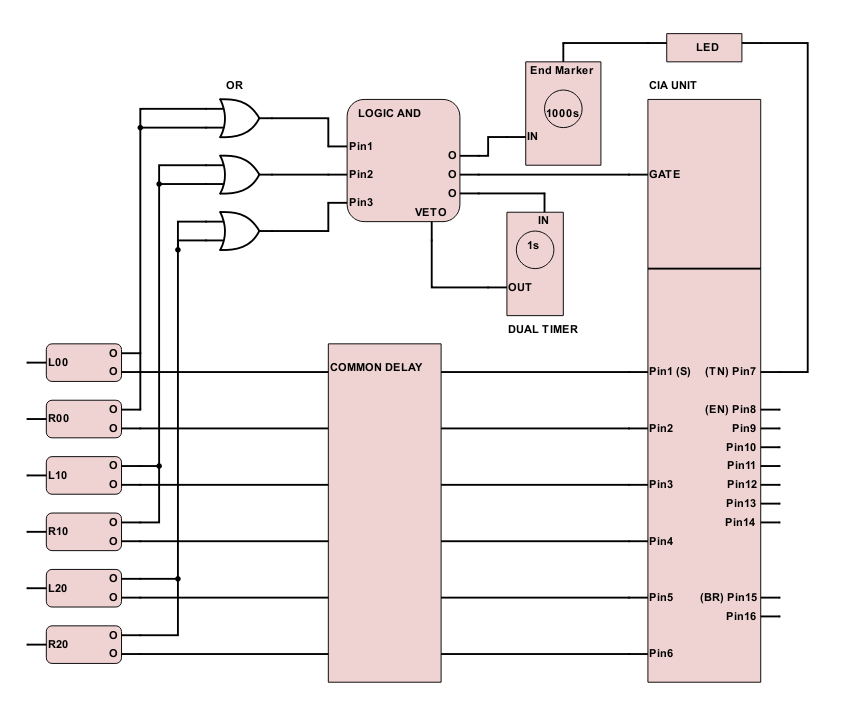
\includegraphics[width=0.8\textwidth]{./SCHEMI/Energy.png} % Include the image placeholder.png
    \caption{\small Rappresentazione schematica del circuito utilizzato per determinare l'energia depositata nei PM da un muone passante.}
	 	\label{fig:circ-energy}
 	\end{center}
 \end{figure}


 \begin{figure}[H]
   \centering
   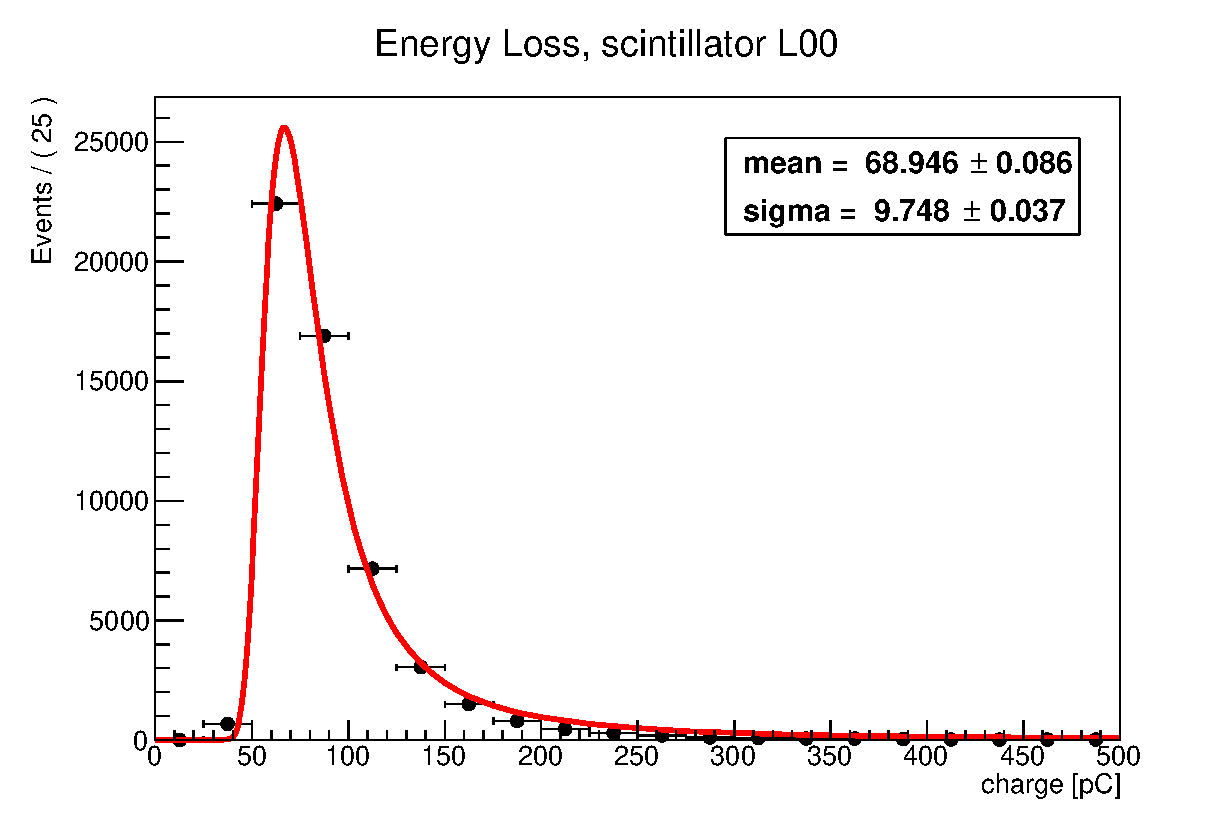
\includegraphics[width=0.9\textwidth]{plots/energy_L00.eps}
   \caption{Distribuzione della carica raccolta da L00. }
   \label{fig:L00_energy}
 \end{figure}

%%%%%%%%%%%%%%%%%%%%%%%%%%%%%%%%%%%%%%%%%%%%%%%%%%%%%%%%%%%%%%%%%%%%%%%%%%%%%%%%%%%%%%%%%%%%%%%%%%%%%%%%%%%%%%%%%%%%%%%%%%%%%%%%%%%%%%%%%%%%%%%%%%%%%%


\begin{thebibliography}{90}             %crea l'ambiente bibliografia
\rhead[\fancyplain{}{\bfseries \leftmark}]{\fancyplain{}{\bfseries
\thepage}}
%%%%%%%%%%%%%%%%%%%%%%%%%%%%%%%%%%%%%%%%%aggiunge la voce Bibliografia
                                        %   nell'indice
\addcontentsline{toc}{chapter}{Bibliografia}
%%%%%%%%%%%%%%%%%%%%%%%%%%%%%%%%%%%%%%%%%provare anche questo comando:
%%%%%%%%%%%\addcontentsline{toc}{chapter}{\numberline{}{Bibliografia}}
\bibitem{pdg} M. Tanabashi et al. (Particle Data Group), Phys. Rev. D 98, 030001 (2018).
\bibitem{Spurio} M. Spurio et al., Particles and Astrophysics; Springer International Publishing Switzerland 2015.
\bibitem{Bendiscioli} G. Bendiscioli, Fenomeni Radioattivi; Springer-Verlag Milan 2013.
\bibitem{Groom} D. Groom, S. Klein, Passage of particles through matter, Eur.Phys. J. C, 15: 163 (2000)
\end{thebibliography}
%%%%%%%%%%%%%%%%%%%%%%%%%%%%%%%%%%%%%%%%%non numera l'ultima pagina sinistra

